
\subsection{Navigation}
In this section, we provide detailed implementation of particle filters localisation (PFL) and novel features used to boost the performance. The Bayesian reasoning of particle filters, however, is not focused in this section.

\vspace{1em}
\begin{algorithm}[H]
\caption{Particle filters localisation} \label{alg:pfl}
\SetAlgoLined
  \KwIn{particles, robot, isConverge}
  \KwOut{estimate, isConverge}  
  updateParticles(particles, robot); \\
  estimate = getEstimation(particles); \\
  \If{isConverge = true \label{alg:condition}}{
  \If{estimate is too different from real robot}{initialise particles; \\ isConverge = false;}
  }
  \Else{
  isConverge = checkConverge(particles); \\
  }
  \Return estimate, isConverge
\end{algorithm}
\vspace{1em}

% implementation details and novelty
We determine the size of particles as 400 via comprehensive experiments, which will be explained later. The implementation of PFL is demonstrated in Algorithm \ref{alg:pfl}. The input to this algorithm includes 400 particles, the real robot and a parameter called {\itshape isConverge} representing the status of these particles. When {\itshape isConverge} equals to 1, these particles are converged and 0 otherwise. The output of this algorithm contains two elements: first is the estimate of the real robot that contains estimated position and orientation; second is the status parameter that commands the robot to continue in exploring the environment to find its location or to move towards the target position.

Initially, the particles are positioned randomly inside a map. We add movement noise and turning noise to the particles using the given functions in the BotSim library. During the localisation process, we first update the particles in terms of their positions and orientations, which is enclosed in the function {\itshape updateParticles()}. To do so, firstly we obtain the scans (sensor readings) of the robot and the particles. These scans are represented as vectors $\mathbf{r}$ and $\mathbf{p}_{i}$, where $i = 1, ..., 400$, for the robot and particles respectively. Secondly, to update each particle's weights, we calculate the difference between the scan of the robot $\mathbf{r}$ and the scan of each particle $\mathbf{p}_{i}$ using the $\ell$1-norm i.e. $d_{i} = ||\mathbf{r} - \mathbf{p_{i}}||_{1}$, and then obtain the new weight for each particle by $$w_{i} = exp(-\frac{d_{i}}{2\sigma^{2}}) + damp$$ where $damp$ is a dampling factor used to prevent the weight from being zero. We use $\ell$1-norm instead of the $\ell$2-norm to compute the difference between two sensor readings because using $\ell$2-norm will make the weights of the particles less informative. For example, when using the $\ell$2-norm, each $d_{i}$ becomes much bigger since the difference is squared for each pair in the two vectors (sensor readings) and accordingly $exp(-\frac{d_{i}}{2\sigma^{2}})$ becomes much smaller and most of them are close to zero. As a consequence, all of the weights of the particles are nearly equal to the dampling factor, which makes the robot harder to match a particle. The $\sigma$ and $damp$ are assigned 3 and 0.01 respectively, which are obtained by running lots of experiments and selecting the optimal setting. Once the weights are computed, we normalise them by  $$w_{i} = \frac{w_{i}}{\sum_{i = 1}^{400}w_{i}} + \alpha$$ where $\alpha = 0.5/400$ is a constant. The reason for adding this constant will be explained later when we describe our resampling process.

The particles with larger weights are closer to the real robot. To do the resampling, we first resort the particles in a weight-decreasing order so the particle with the largest weight is positioned at the first and then we redistribute these particles. The particle with the max weight is copied for $n_{i} = w_{i}\times N$ times where $N=400$, and we repeat the same step for each particle in the queue until the number of the new particles is equal to 400 i.e. $\sum n_{i}=400$. However, during this process, we found that the number could not reach to 400 because many $n_{i}$ equaled to zero since $w_{i}\times N < 0.5$ (we used round to get an integer). Therefore, we add the constant $0.5/N$ to ensure the resulting $n_{i}$ satisfies $n_{i}\ge 0.5$ such that $n_{i}$ can be rounded to 1 rather than 0.

\begin{figure}[h]
\centering
  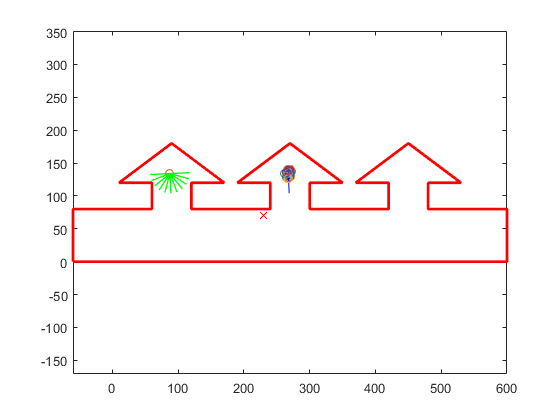
\includegraphics[scale=0.6]{symm}
  \caption{Robot in a symmetric environment causing the symmetric ambiguity problem.}
  \label{fig:symm}
\end{figure}

The {\itshape estimate} of the real robot that contains the position and orientation information is computed by separately averaging the positions and orientations of the new particles. After this, we check whether the particles were converged previously i.e. we go to Line \ref{alg:condition} in Algorithm \ref{alg:pfl}. There are two situations that will happen: (\textbf{1}) If they were converged, we need to check whether the obtained {\itshape estimate} matches the real robot or not. This step is necessary because if the map is somewhat symmetric as shown in Fig.\ref{fig:symm}, the particles were very likely to converge in a wrong place although the sensor readings were consistent with the robot's. We compare the {\itshape estimate} with the real robot in this way: suppose the sensor readings of the {\itshape estimate} are $\mathbf{e}$ and those of the real robot are $\mathbf{r}$, the difference between them is computed by $df=||\mathbf{e}-\mathbf{r}||_{1}$. If $df$ is bigger than a threshold, which means the {\itshape estimate} is inaccurate and the particles converged in an incorrect place, all the particles will be randomly positioned again and the status parameter {\itshape isConverge} will be set to {\itshape false}. (\textbf{2}) If the particles were not converged, they need to be checked by the function {\itshape checkConverge()}. With the observation that if the particles are converged, they will look compact in the 2D map. We thus use a statistical method to check the convergence: we calculate the 2 by 2 covariance matrix (CovMat) based on the positions $(x,y)$ of the particles and obtain the corresponding eigenvalues of the CovMat; these two eigenvalues describe the spread of the particles and how tight they are; we define the particles being converged if and only if the sum of the eigenvalues is lower than an experimentally determined threshold. By performing this localisation process, the particles are able to accurately find its location in a known map and the symmetric ambiguity is possible to be eliminated.

% how to select an optimal size
In order to select an optimal value as the size of the particle filters, we performed substantial experiments in which the size ranged from 100 to 1000 with an increment of 100. Thus there were totally 10 candidate values. We fixed the starting position of the real robot at $(20,20)$ and the target position at $(80,80)$ using the first map provided as shown in Fig.\ref{fig:experiment}. The distance between these two positions is sufficient for the particles to get converged. To judge the performance of the PFL with different size settings, we designed three criteria: {\itshape distance error} ($e$), {\itshape convergence time} ($t$) and {\itshape standard deviation} ($s$). The definitions of these three criteria are specified as follows:

\begin{itemize}
  \item Distance error ($e$): it is defined as the Euclidean distance between the target position and the final robot position.
  \item Convergence time ($t$): it calculates the time (in seconds) that the particles require to get converged.
  \item Standard deviation ($s$): it defines how accurate the estimated position is after the particles get converged and can represent the stability of the algorithm. The mathematical expression is as follows: suppose after the robot finds its location it requires $N$ steps to get stopped, denote the 2D position of the robot at each time step $i$ as $P^{r}_{i}$ and the estimation as $P^{e}_{i}$, the standard deviation $s$ is computed as $s = \sqrt{ \frac{1}{N}\sum_{i=1}^{N}||P^{r}_{i} - P^{e}_{i}||^{2} }$.
\end{itemize}

For each size setting, we ran 100 experiments where we computed the $e$, $t$ and $s$ for each and finally we averaged them as the output. The results are plotted in Fig.\ref{fig:sizedeter}, where the lower the values are, the better the performance is. It can be seen that the convergence time (green) increases as the size of the particle filters increases. On the distance error (blue) and the standard deviation (red), the algorithm with sizes from 300 to 1000 produces comparable results. Therefore, from this graph we could not decide which size is the optimal. To overcome this problem, we combined these three criteria to form a penalty-based criterion that can be used to distinguish one with the relatively best performance from the rest. We defined this criterion as {\itshape penalty-based score}, which was computed by $$psc = \frac{1}{e+1.5t+s}$$ The constant added before the $t$ aims to increase the weight of the convergence time such that the size that causes longer time for the particles to converge is less wanted since it decreases the score. As a result, the new ranking is more clear and the size equal to 400 has the best score as shown in Fig.\ref{fig:scorecompute}. Thesefore, we selected 400 as the optimal size.

% novel features
By running this algorithm to localise the robot in the simulation, we obtained promising results where the average distance from the target was always less than 3. Here we summarise the novel features used in this algorithm:

\begin{itemize}
  \item $\ell$1-norm based weights updating function.
  \item the $\alpha$ constant that is added when normalising the weights for the particles.
  \item a re-validation method to measure whether the obtained estimate is correct or not.
  \item a statistical method to determine the convergence condition.
  \item a penalty-based score to help select the optimal size for particle filters.
\end{itemize}

\begin{figure}[h]
\centering
  \begin{subfigure}{0.48\textwidth}
  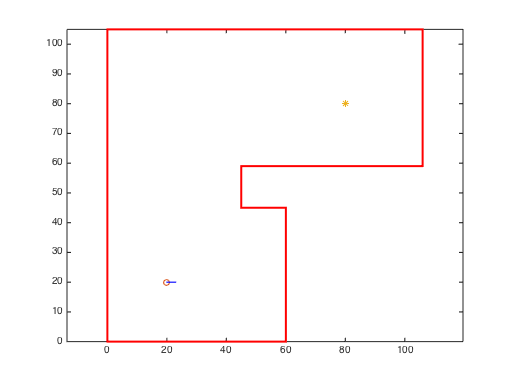
\includegraphics[scale=0.5]{experiment}
  \caption{}
  \label{fig:experiment}
  \end{subfigure}
  \begin{subfigure}{0.48\textwidth}
  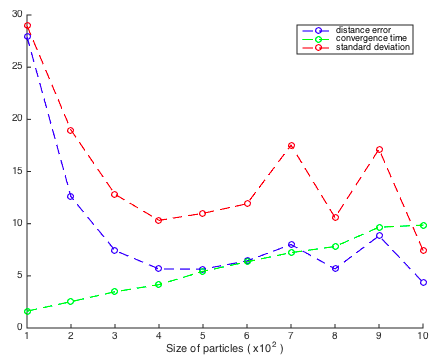
\includegraphics[scale=0.5]{sizedetermine}
  \caption{}
  \label{fig:sizedeter}
  \end{subfigure}
  \begin{subfigure}{0.48\textwidth}
  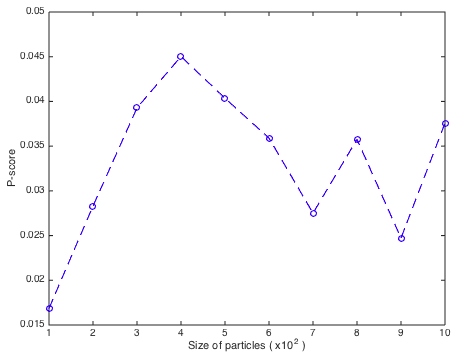
\includegraphics[scale=0.5]{scorecompute}
  \caption{}
  \label{fig:scorecompute}
  \end{subfigure}
  \caption{Experiments to select an optimal size of particle filters.}
\end{figure} 


\FloatBarrier